%
% ****
\chapter{Leaky Integrate and Fire und simulative Modelle neuronaler Netze}
\label{chap:lif}
% ****
%

	Um biologische neuronale Netze zu simulieren und nutzbar zu machen, bedarf es verschiedener Modelle und Algorithmen. Dieses Kapitel stellt das \textit{Leaky Integrate and Fire (LIF)} - Modell vor, welches zur Berechnung des Membranpotentials einer internen Nervenzelle dient. Da es sich hier um eine lineare Differenzialgleichung erster Ordnung handelt, werden darüber hinaus numerische Berechnungsmethoden vorgestellt, welche ebenfalls implementiert werden. Weiterhin wird auf die Berechnung der Synapsenströme und Übersetzung der Sensorpotentiale eingegangen und ein simulatives Modell des neuronalen Netzes vorgestellt.

% ***
\section{Herleitung des Leaky Integrate and Fire - Modells}
\label{sec:lif_model}
% ***
	Grundsätzlich wird in der Natur beobachtet, dass die neuronale Dynamik als Summationsprozess gefolgt von einer kurzfristigen Entladung des Aktionspotentials beschrieben werden kann. Die Entladung erfolgt hierbei immer ab einem gewissen Wert, welcher als Schwellwert $\vartheta$ beschrieben wird. Bei Überschreitung dieses Grenzwertes \glqq feuert\grqq{} die Nervenzelle und Informationen gelangen über Synapsen und Gap-Junctions zu nahegelegenen Neuronen.
	
	Um dieses Verhalten zu modellieren, wird der Zellkern genauer betrachtet. Dieser ist mit einer Zellmembran umgeben, welche als guter Isolator dient. Bei anliegenden Strömen $I_{Stimuli}$, $I_{Syn}$ oder $I_{Gap}$ wird die elektrische Ladung $q = \int I(t')dt'$ die Membran aufladen. Die Zellmembran handelt analog eines Kondensators mit Kapazität $C_m$. Da jedoch in der Natur kein perfekter Kondensator existiert, verliert die Zellmembran über die Zeit minimal elektrische Ladung. Daher wird dem Kondensator im Ersatzschaltbild ein Leckwiderstand $R$ parallel geschaltet. Um das beobachtete Ruhepotential $U_{Leak}$ nach einem Feuer-Event oder bei keinem Eingang wiederherzustellen, wird eine Batterie in Reihe mit dem Widerstand $R$ geschaltet.
	
	Technisch lässt sich dieses Verhalten als ein elektrisches Ersatzschaltbild wie in Abbildung \ref{cic:lif} darstellen (siehe \cite{NeuronalDynamics} Kap. 1.3.1).
	\begin{figure}
		\centering
		\begin{circuitikz}
			\draw	
			%(0,0) to [short, *-*] (5,0)
			(0,4) to [short, o-*] (1,4)
			to [generic, l=$R$] (1,2)
			to [battery1, l=$U_{Leak}$] (1,0)
			to [short, -*] (1,0)
			to [short, -o] (0,0)
			
			(1,4) to [short, i_>=$I$] (3,4)
			to [short, -*] (3,4)
			to [C, l=$C_m$] (3,0)
			to [short, -*] (3,0)
			to [short, -*] (1,0)
			
			(3,4) to [short, -o] (4,4)
			(3,0) to [short, -o] (4,0)
			(4,0) to [open, v_<=$U$] (4,4);
		\end{circuitikz}
		\caption{Ersatzschaltbild der Zellmembran}
		\label{cic:lif}
	\end{figure}
	Um nun eine geeignete Differenzialgleichung herzuleiten, wird zuerst das erste Kirchhoffsche Gesetz angewendet
	\begin{align}
		\label{eq:lif_current}
		I = I_R + I_C\text{.}
	\end{align}
	Der Strom $I_R$ ist einfach durch das Ohmsche Gesetz wie folgt zu berechnen
	\begin{align}
		\label{eq:lif_IR}
		I_R = \frac{U_R}{R} = \frac{U - U_{Leak}}{R}\text{.}
	\end{align}
	Der Strom $I_C$ wird durch die Definition eines Kondensators $C_m = \tfrac{q}{U}$ zum kapazitiven Strom 
	\begin{align}
		\label{eq:lif_IC}
		I_C = \frac{dq}{dt} = C_m \frac{dU}{dt}\text{.}
	\end{align}
	Hierbei steht $q$ für die elektrische Ladung und $U$ für die anliegende Spannung.
	
	Einsetzen von \eqref{eq:lif_IR} und \eqref{eq:lif_IC} in \eqref{eq:lif_current} ergibt
	\begin{align}
		\label{eq:lif_I}
		I = \frac{U - U_{Leak}}{R} + C_m\frac{dU}{dt}\text{.}
	\end{align}
	Wird diese Gleichung mit $R$ multipliziert und umgestellt, bildet sich die folgende lineare Differenzialgleichung erster Ordnung:
	\begin{align}
		\label{eq:lif_nd}
		R C_m \frac{dU}{dt} = (U_{Leak} - U) + R I\text{.}
	\end{align}
	Der Strom $I$ wird als Eingangsgröße verstanden und im weiteren Verlauf als $I_{in}$ betitelt. Nach Division durch $RC$ und Einführung des Leitwerts $G_{Leak} = \tfrac{1}{R}$ entsteht die gewollte Form:
	\begin{align}
		\label{eq:lif}
		\frac{dU}{dt} = \frac{G_{Leak}(U_{Leak} - U) + I_{in}}{C_m}\text{.}
	\end{align}
	In dieser Gleichung stehen die Variablen $G_{Leak}$, $U_{Leak}$ und $C_m$ für Parameter der betrachteten Nervenzelle, während $I_{in}$ stellvertretend für alle eingehenden Ströme aus Stimuli, chemischen Synapsen und Gap-Junctions steht
	\begin{align}
		\label{eq:lif_current_in}
		I_{in} = \sum_{i = 1}^{n}{I_{Stimuli}} + \sum_{i = 1}^{n}{I_{Syn}} + \sum_{i = 1}^{n}{I_{Gap}}\text{.}
	\end{align}
	Die Implementierung dieser Gleichungen und den entsprechenden numerischen Lösungsverfahren findet sich in Abschnitt \ref{sec:lif_neuro}. Ein beispielhafter Spannungsverlauf bei einem konstanten, positiv einfließendem Strom $I_{in}$ wird in Abbildung \ref{fig:simple_lif} dargestellt.
	\begin{figure}[h]
		\centering
		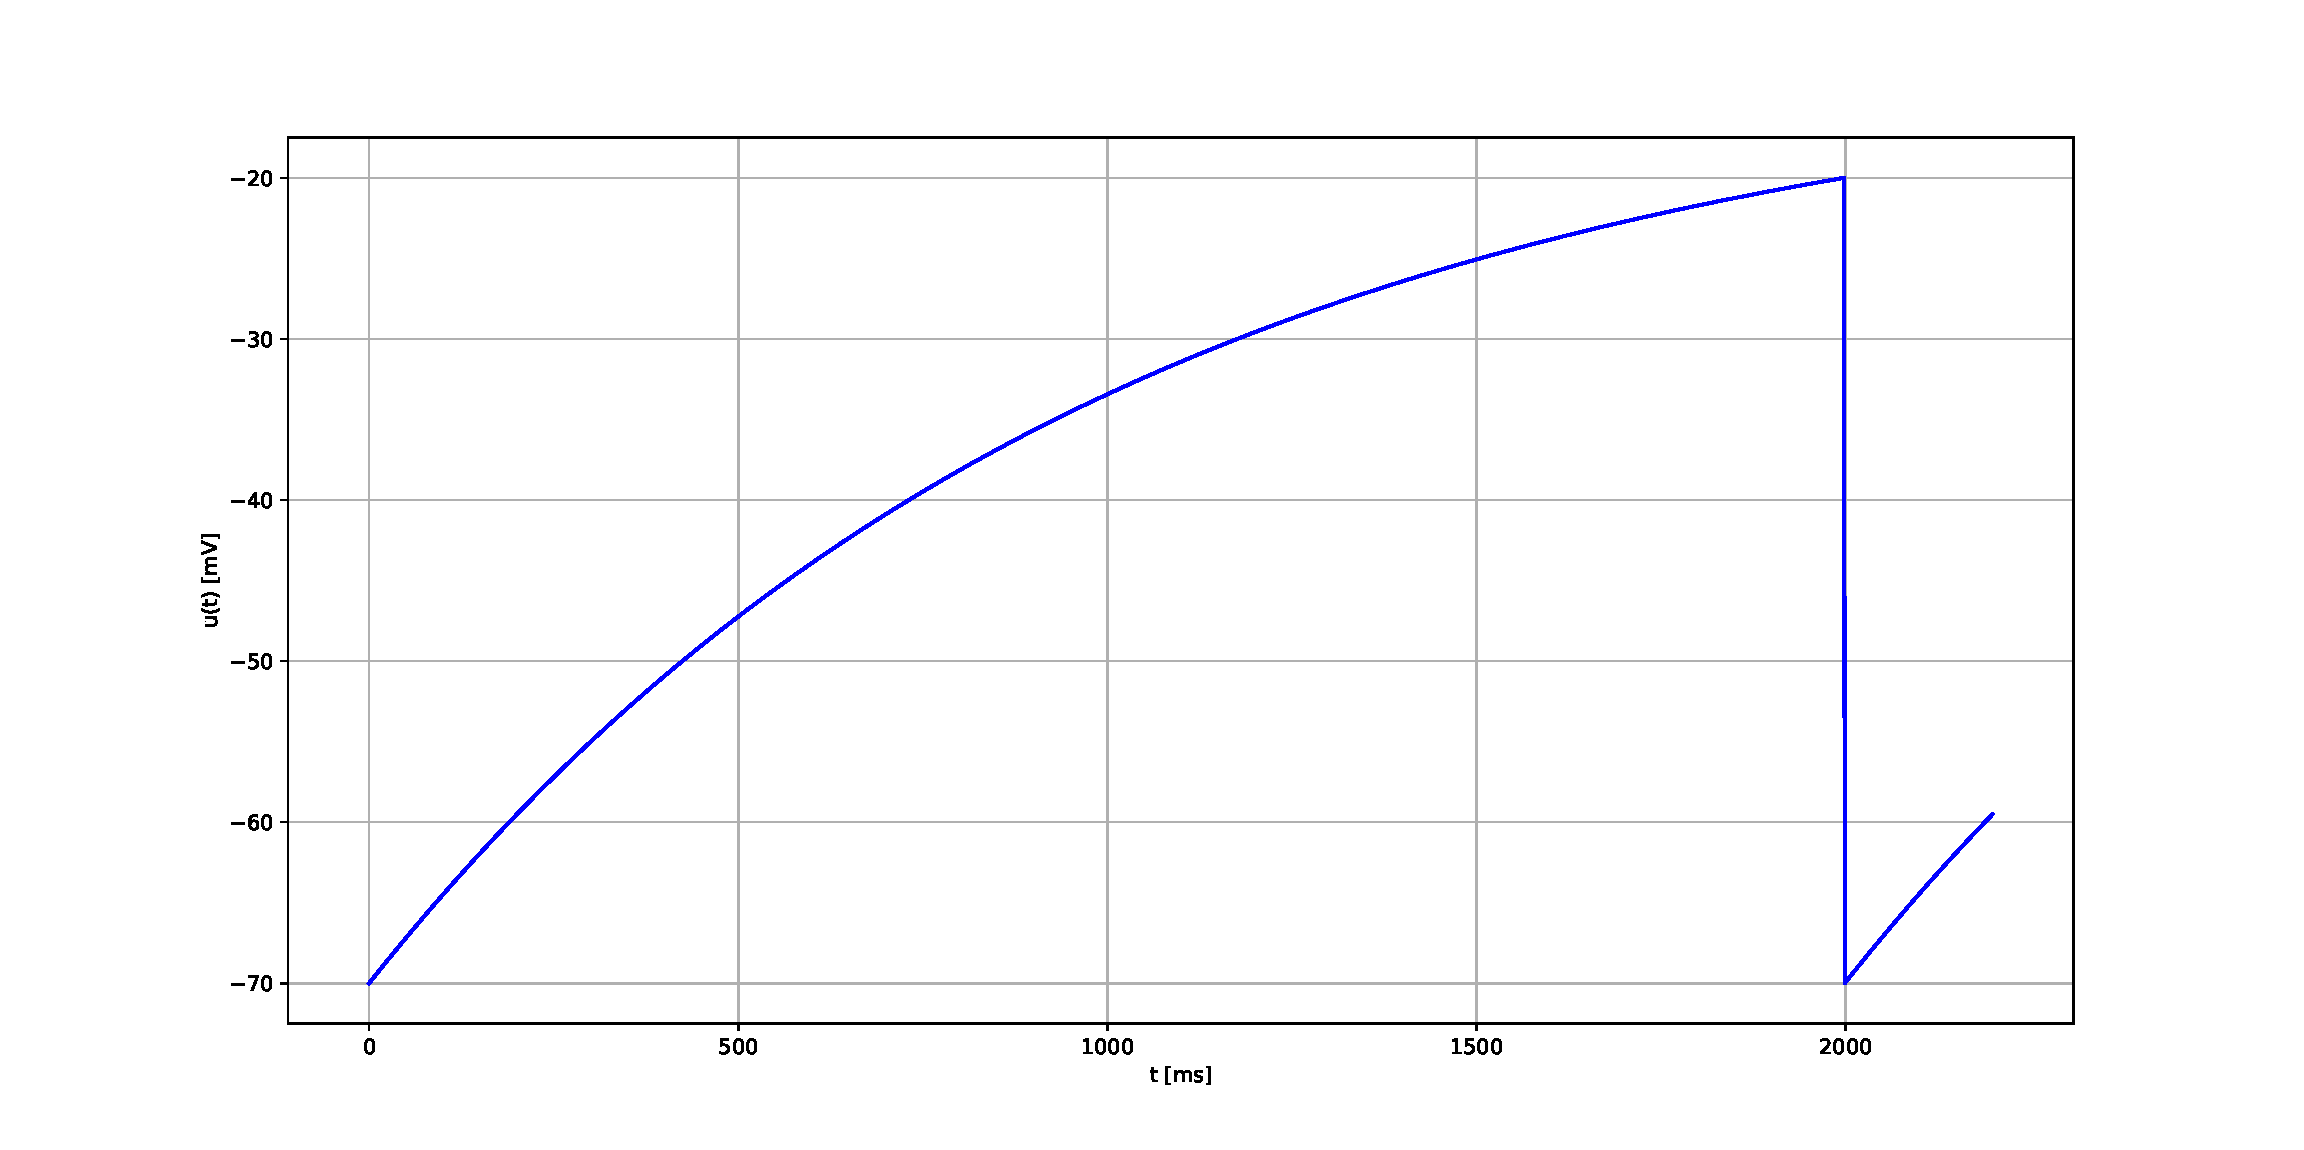
\includegraphics[width=14cm]{figures/chap_lif/Simple_LIF.pdf}
		\caption{Grafische Darstellung des Membranpotentials durch das \textit{LIF} - Modell.}
		\label{fig:simple_lif}
	\end{figure}
	Die anliegenden Synapsenströme sind durch folgenden formularen Zusammenhang zu berechnen \cite{WormLevelRL}:
	\begin{align}
		\label{eq:chem_syn_current}
		I_{Syn} = \frac{w}{1 + \e^{\sigma(u_{pre} + \mu)}}(E - u_{post})\text{.}
	\end{align}
	Synapsenströme sind grundsätzlich von den pre- und postsynaptischen Potentialen der jeweiligen Nervenzellen $u_{pre}$ und $u_{post}$ abhängig. Weiterhin können diese chemischen Synapsen exzitatorisch oder inhibitorisch wirken. Diese Eigenschaft wird durch das sog. Nernstpotential $E\in[-90\text{ mV}, 0\text{ mV}]$ beschrieben. Weitere Größen dieser Gleichung bilden die Kreisfrequenz $w$, die Standardabweichung $\sigma$ und der Erwartungswert $\mu$.
	
	Gap-Junctions bilden die Ausnahme, denn sie dienen als Ausgleichsglied und wirken bidirektional. Ihr Strom wird wie folgt berechnet:
	\begin{align}
		\label{eq:gap_syn_current}
		I_{Gap} = \hat{w}(u_{post} - u_{pre})\text{.}
	\end{align}
	Für die Berechnung des Gap-Junction Stroms benötigt es ebenfalls das pre- und postsynaptische Potenzial der jeweiligen Nervenzellen $u_{pre}$ und $u_{post}$, sowie die Kreisfrequenz $\hat{w}$.
	
% ***
\section{Anwendung auf Modelle neuronaler Netze}
\label{sec:lif_neuro}
% ***
	Durch das im vorherigen Kapitel beschriebene \textit{LIF} - Modell ist es möglich, interne Vorgänge eines neuronalen Netzes zu beschreiben und zu simulieren. Dies setzt jedoch einen konstanten Eingang der vier Sensorneuronen durch äußere Stimuli voraus. Diese Rezeptoren sind in der Lage, äußere Einflüsse wie bspw. Licht- oder Berührungsintensität in eine für das neuronale Netz verständliche Größe zu übersetzen. Wie bereits eingangs erwähnt, existiert ein Aktionsraum $A\in[-70\text{ mV}, -20\text{ mV}]$, wobei $-70\text{ mV}$ als Ruhespannung und $-20\text{ mV}$ als Aktionspotential wahrgenommen wird. Aufgabe der vier Sensor-Neuronen \textit{PVD, PLM, AVM und ALM} ist es folglich, eingehende Größen entsprechend auf den gegebenen Aktionsraum $A$ zu übersetzen.
	
	In dem bereits thematisierten Schaubild nach Lechner et al (Abbildung \ref{fig:01_TW-Circuit}) werden jeweils zwei Sensorneuronen für einen Eingang genutzt, da zwischen positiven und negativen Eingangsgrößen unterschieden wird. \textit{PLM und AVM} bilden das primäre Sensorpaar für die ausschlaggebendste Eingangsgröße (inverses Pendel: Winkel $\varphi$), \textit{PVD und ALM} bedienen eine sekundäre Eingangsgröße (inverses Pendel: Winkelgeschwindigkeit $\dot{\varphi}$ oder Wagenposition $x$). Diese Wahl beruht auf der internen Verschaltung des Netzwerks durch Synapsen und Gap-Junctions.
	
	Um nun die jeweiligen Größen durch die Sensorneuronen zu übersetzen, werden folgende Funktionen für die jeweils positive und negative Sensorneurone $S_{positiv}$ und $S_{negativ}$ angenommen:
	\begin{align}
		\label{eq:sensor_translation_p}
		S_{positiv} &:= \begin{cases}-70\text{ mV} & x\leq 0\\-70\text{ mV} + \frac{5\text{ mV}}{x_{min}}x & 0 < x \leq x_{min} \\-20\text{ mV} & x > x_{max}  \end{cases}\\
		\label{eq:sensor_translation_n}
		S_{negativ} &:= \begin{cases}-70\text{ mV} & x\geq 0\\-70\text{ mV} + \frac{50\text{ mV}}{x_{min}}x & 0 > x \geq x_{min} \\-20\text{ mV} & x < x_{max}  \end{cases}
	\end{align}
	$x\in[x_{min}, x_{max}]$ ist eine messbare, dynamische Systemvariable, welche in den gegebenen Grenzen $x_{min} $ und $x_{max}$ auftritt. Lediglich eine Fallunterscheidung wird getroffen: nimmt $x$ einen positiven Wert an, wird Sensorneurone $S_{positiv}$ aktiviert, bei negativem $x$-Wert, agiert die Sensorneurone $S_{negativ}$.
	
	Analog lässt sich dieser Zusammenhang auf die beiden Motorneuronen \textit{REV} und \textit{FWD} übertragen. Hier werden die Signale der internen Nervenzellen \textit{AVA} und \textit{AVB} auf interpretierbare Größen in die Außenwelt übersetzt. Biologisch kann dies ein Nervenimpuls sein, welcher eine spezielle Muskelgruppe anspricht oder einen Reflex auslöst. In der oben genannten Simulationsumgebung des inversen Pendels entspricht der Ausgang des Netzwerks entweder einer diskreten Vorwärts- oder einer Rückwärtsbewegung. Genaueres zu der Interaktion mit dem genannten Simulationskonstrukt im Kapitel \ref{chap:imp}.

% ***
\section{Zuverlässigkeit und Limitationen}
\label{sec:lif_lim}
% ***
	Das \textit{LIF} - Modell ist stark vereinfacht und zeigt die grundsätzlichen Eigenschaften des Membranpotentials auf. Es erfolgt eine Integration der anliegenden Ströme und eine simple Rücksetzung des Aktionspotentials nach Überschreitung des Schwellenwertes $\vartheta$ auf das Ruhepotential $U_{Leak}$.
	
	Zur weiteren Analyse eines neuronalen Netzwerks besonders im Bereich der Biologie und Biochemie werden daher detailliertere Modelle angewendet, um biologische Effekte in verschiedenen Zelltypen zu berücksichtigen. Jedoch eignet sich das hier angewendete Modell sehr gut zur Analyse der gegebenen Nervenzellen. Das \textit{LIF} - Modell ist in der Lage, sog. Feuer-Events bei der Überschreitung des genannten Schwellenwertes exakt zu ermitteln und liefert somit eine grundlegende Zeitbasis für die Simulationsumgebung.
	
	Da das biologische neuronale Netzwerk qualitativ betrachtet werden soll und eine spätere Optimierung durch Parameterfindung und Gewichtung erfolgt, wird das \textit{LIF} - Modell weiterhin verwendet.

% ***
\section{Implementierung}
\label{sec:lif_imp}
% ***
	Zur Implementierung des \textit{LIF} - Modells wird die Programmiersprache \texttt{Python} verwendet.  Angelehnt an die Formeln aus Abschnitt \ref{sec:lif_model} kann ein einfacher Algorithmus implementiert werden. Der gesamte Code befindet sich im zugehörigen GitHub-Repository\footnote{https://github.com/J0nasW/BA}.
	
	Da sich in der Berechnung der Membranpotentiale eine lineare Differenzialgleichung erster Ordnung ergibt (siehe \eqref{eq:lif}), muss diese entsprechend numerisch gelöst werden. Die Lösung kann durch das Euler-Verfahren sowie durch die Methode nach Runge-Kutta gefunden werden, wobei letztere (4. Ordnung) deutlich genauer ist. Folgende numerische Lösungsverfahren wurden dem Buch \glqq Nonlinear Dynamics and Chaos\grqq{} \cite{NonlinearDynamics} entnommen:
	\subsection{Numerisches Lösungsverfahren nach Euler}
		Gegeben sei eine Differenzialgleichung der Form $\dot{x} = f(x)$ mit der Bedingung $x = x_0$ bei $t = t_0$. Man finde einen Weg, um die Lösung $x(t)$ zu approximieren.\\
		Weiterhin sollte die Schrittweite $\Delta t$ bekannt sein sowie die Anzahl der Zeitschritte $T$. Somit lässt sich die Differenzialgleichung numerisch lösen:
		\begin{align}
			\label{eq:euler}
			x_{n+1} = x_n + f(x_n) \Delta t
		\end{align}
	\subsection{Numerisches Lösungsverfahren nach Heun}
		Gegeben sei ebenfalls eine Differenzialgleichung der Form $\dot{x} = f(x)$ mit der Bedingung $x = x_0$ bei $t = t_0$. Man finde einen Weg, um die Lösung $x(t)$ zu approximieren.\\
		Weiterhin sollte die Schrittweite $\Delta t$ bekannt sein sowie die Anzahl der Zeitschritte $T$. Somit lässt sich die Differenzialgleichung numerisch lösen:
		\begin{align}
			\label{eq:erw_euler}
			\tilde{x}_{n+1} &= x_n + f(x_n) \Delta t\\
			x_{n+1} &= x_n + \tfrac{1}{2}[f(x_n) + f(\tilde{x}_{n+1})]\Delta t
		\end{align}
		Dieses Verfahren ermöglicht eine genauere Approximation als die einfache Euler-Methode bei gleichbleibender Schrittweite. Der Fehler $E = |x(t_n)-x_n|$ wird kleiner.
	\subsection{Numerisches Lösungsverfahren nach Runge-Kutta 4. Ordnung}
		Gegeben sei eine Differenzialgleichung der Form $\dot{x} = f(x)$ mit der Bedingung $x = x_0$ bei $t = t_0$. Man finde einen Weg, um die Lösung $x(t)$ zu approximieren.\\
		Weiterhin sollte die Schrittweite $\Delta t$ bekannt sein sowie die Anzahl der Zeitschritte $T$. Somit lässt sich die Differenzialgleichung numerisch lösen:
		\begin{align}
			\begin{split}
			\label{eq:rungekutta}
			k_1 &= f(x_n) \Delta t\\
			k_2 &= f(x_n + \tfrac{1}{2} k_1) \Delta t\\
			k_3 &= f(x_n + \tfrac{1}{2} k_2) \Delta t\\
			k_4 &= f(x_n + k_3) \Delta t\\
			\end{split}\\[10pt]
			x_{n+1} &= x_n + \tfrac{1}{6} (k_1 + 2 k_2 + 2 k_3 + k_4)
		\end{align}
		Dieses Verfahren ermöglicht eine genauere Approximation als die Euler-Methoden bei gleichbleibender Schrittweite. Der Fehler $E = |x(t_n)-x_n|$ wird signifikant kleiner. Diese Methode erfordert jedoch eine höhere Rechenzeit und ist daher nur bei ausreichender Leistung anzuwenden.
	Anwendung des Lösungsverfahrens nach Runge-Kutta (Gleichung \eqref{eq:rungekutta}) auf die Funktion \eqref{eq:lif} resultiert in folgende Berechnung, welche direkt implementiert werden kann:
	\begin{equation}
	\begin{split}
		\label{eq:runkgekutta_nn}
		k_1 &= \frac{G_{leak} (U_{leak} - u(t)) + (I_{Stimuli} + I_{Syn} + I_{Gap})}{C_m} \Delta t\\
		k_2 &= \frac{G_{leak} (U_{leak} - (u(t) + \tfrac{1}{2} k_1)) + (I_{Stimuli} + I_{Syn} + I_{Gap})}{C_m} \Delta t\\
		k_3 &= \frac{G_{leak} (U_{leak} - (u(t) + \tfrac{1}{2} k_2)) + (I_{Stimuli} + I_{Syn} + I_{Gap})}{C_m} \Delta t\\
		k_4 &= \frac{G_{leak} (U_{leak} - (u(t) + k_3)) + (I_{Stimuli} + I_{Syn} + I_{Gap})}{C_m} \Delta t
	\end{split}
	\end{equation}
	Rekursive Berechnung der vier Koeffizienten führt zum neuen Membranpotential und entsprechend zu der Information, ob die internen Nervenzellen \textit{AVA} oder \textit{AVB} gefeuert haben:
	\begin{align}
		\label{eq:runkgekutta_erg}
		u_{t+1}(t) &= u(t) + \tfrac{1}{6} (k_1 + 2 k_2 + 2 k_3 + k_4).
	\end{align}
	Um diese Funktion im Gesamtcode später aufrufen zu können, wird ein Python-Script (\texttt{modules/lif.py}) erstellt. Dieses enthält neben der Funktion zur Berechnung des Membranpotentials auch die der Berechnung von Synapsen- und Gap-Junction-Strömen.
	
	Im weiteren Verlauf werden Algorithmen zur Suche der entsprechenden Parameter des biologischen neuronalen Netzes eingeführt. In diesen wird eine Funktion \texttt{compute} implementiert, welche das Modul \texttt{lif.py} aufruft. Um eine effiziente Berechnung der Membranpotentiale und Synapsen- bzw. Gap-Junction Ströme zu gewährleisten, wird die Funktion wie folgt aufgebaut:
	\begin{algorithm}
		\SetKwInOut{Input}{Input}
		\SetKwInOut{Output}{Output}
		
		\Input{$\boldsymbol{x}, \boldsymbol{u}, \boldsymbol{A}, \boldsymbol{B}, \boldsymbol{C_m}, \boldsymbol{G_{Leak}}, \boldsymbol{U_{Leak}}, \boldsymbol{\sigma}, \boldsymbol{w}, \boldsymbol{\hat{w}}$}
		\Output{$\boldsymbol{x}, \boldsymbol{u}, \boldsymbol{fire}, \boldsymbol{I_{Syn}}, \boldsymbol{I_{Gap}}$}
		
		\For{i $\leftarrow$ 1 \textbf{to} 4}{
			\For{j $\leftarrow$ 1 \textbf{to} 4}{
				\uIf{$\boldsymbol{A_{i,j}} == 1$}{
					I\_inter$_{i,j}$ = I\_syn\_calc($x[i], x[j], E_{in}, w[k], \sigma[k], \mu$)\\
					k $\leftarrow$ k + 1
				}
				\uElseIf{$\boldsymbol{A_{i,j}} == 2$}{
					I\_inter$_{i,j}$ = I\_syn\_calc($x[i], x[j], E_{ex}, w[k], \sigma[k], \mu$)\\
					k $\leftarrow$ k + 1
				}
				\Else{
					I\_inter$_{i,j}$ = 0
				}
			
				\uIf{$\boldsymbol{B_{i,j}} == 1$}{
					I\_sensor$_{i,j}$ = I\_syn\_calc($u[i], u[j], E_{in}, w[k], \sigma[k], \mu$)\\
					l $\leftarrow$ l + 1
				}
				\uElseIf{$\boldsymbol{B_{i,j}} == 3$}{
					I\_sensor$_{i,j}$ = I\_gap\_calc($u[i], x[j], \hat{w}[k]$)\\
					m $\leftarrow$ m + 1
				}
				\Else{
					I\_sensor$_{i,j}$ = 0
				}
			}
		}
		\For{i $\leftarrow$ 0 \textbf{to} 4}{
			I\_inter = I\_inter.sum(axis = 0)\\
			I\_sensor = I\_sensor.sum(axis = 0)\\
			x[i], fire[i] = U\_neuron\_calc($x[i], I\_inter[i], I\_sensor[i], C_m[0,i], G_{Leak}[0,i], U_{Leak}[0,i], v, \Delta t$)
			
		}
		\KwRet{$\boldsymbol{x}, \boldsymbol{u}, \boldsymbol{fire}, \boldsymbol{I_{Syn}}, \boldsymbol{I_{Gap}}$}
		\caption{compute}
	\end{algorithm}\\
	Die Vektoren $\boldsymbol{x}$ und $\boldsymbol{u}$ spiegeln die aktuellen Membranpotentiale der jeweiligen Nervenzellen wider:
	\begin{align}
		\boldsymbol{x} &= \begin{pmatrix}AVA & AVD & PVC & AVB\end{pmatrix}\text{ und}\\
		\boldsymbol{u} &= \begin{pmatrix}PVD & PLM & AVM & ALM\end{pmatrix}\text{.}
		\label{eq:xu}
	\end{align}
	Vektor $\boldsymbol{x}$ beschreibt das Membranpotential interner Nervenzellen, Feuer-Events der Neuronen \textit{AVA} und \textit{AVB} sind später von Interesse. Das Potential der Eingangsneuronen $\boldsymbol{u}$ wird durch die Berechnungsvorschriften \eqref{eq:sensor_translation_p} und \eqref{eq:sensor_translation_n} je nach Sensordaten gesetzt.
	
	Matrizen $A$ und $B$ werden als Transitionsmatrizen genutzt, um die Verbindungen der Nervenzellen im neuronalen Netz zu beschreiben.
	\begin{align}
		\label{eq:mat_A}
		A &= \bordermatrix{
		\quad\Rsh& AVA & AVD & PVC & AVB \cr
			AVA &  0  &  0  &  1  &  1  \cr
			AVD &  2  &  0  &  2  &  0  \cr
			PVC &  0  &  2  &  0  &  2  \cr
			AVB &  1  &  1  &  0  &  0  \cr
		}
	\end{align}
	beschreibt Verbindungen innerhalb der internen Nervenzellen. Dabei stehen die Ziffern $[0,1,2]$ für folgende Verbindungen:
	\begin{align*}
		0 &: \text{Keine Verbindung zwischen Neuronen }A_i\text{ und } A_j\\
		1 &: \text{Inhibitorische Verbindung zwischen Neuronen }A_i\text{ und }A_j\\
		2 &: \text{Exzitatorische Verbindung zwischen Neuronen }A_i\text{ und }A_j.
	\end{align*}
	Die Matrix
	\begin{align}
		\label{eq:mat_B}
		B &= \bordermatrix{
		\quad\Rsh& AVA & AVD & PVC & AVB \cr
			PVD &  0  &  1  &  1  &  0  \cr
			PLM &  1  &  1  &  3  &  0  \cr
			AVM &  0  &  3  &  1  &  1  \cr
			ALM &  0  &  1  &  1  &  0  \cr
		}
	\end{align}
	beschreibt analog die Verbindungen der Sensor-Neuronen mit den internen Nervenzellen. Verbindungen werden zwischen diesen Typen von Nervenzellen nur durch inhibitorische Synapsen und Gap-Junctions hergestellt. Die Ziffern $[0,1,3]$ haben folgende Bedeutung:
	\begin{align*}
		0 &: \text{Keine Verbindung zwischen Neuronen }B_i\text{ und } B_j\\
		1 &: \text{Inhibitorische Verbindung zwischen Neuronen }B_i\text{ und }B_j\\
		3 &: \text{Verbindung durch Gap-Junction zwischen Neuronen }B_i\text{ und }B_j.
	\end{align*}
	Durch diese Vorschriften ist eine Implementierung des gegebenen neuronalen Netzes möglich und die Berechnung essenzieller Größen durch einfache Matrixoperationen zu realisieren.\\
	Ein entsprechendes Modell des neuronalen Netzes lässt sich durch den Zusammenhang
	\begin{align}
		\dot{x} = A\boldsymbol{x} + B\boldsymbol{u}
	\end{align}
	beschreiben. Für die spätere Implementierung sind die gezeigten Gleichungen und Systembeschreibungen essenziell und werden im weiteren Verlauf wieder aufgegriffen.

%%% Local Variables: 
%%% mode: latex
%%% TeX-master: "main"
%%% End: 
